%Author: Jackson Perry
\section{Linear Regression}

In a data set involving two variables, we can attempt to map a relation between them using linear regression. This technique can be used to model such a relation through its generation of a linear equation. In linear regression, one variable is considered to be the independent variable and the other the dependent variable. We typically denote the dependent, or response, variable as $y$ and the independent, or explanatory, variable as $x$. Thus we can generate the linear equation

\begin{equation}
    y = \beta x
\end{equation}

where $\beta$ is a real coefficient denoting the slope of the line. A more commonly used function includes an additional constant term ($\alpha$) allowing the translation of the line turning it into an affine function. Adding $\alpha$ to Equation 2.4 yields

\begin{equation}
    y = \alpha + \beta x
\end{equation}

It is important to note that while a strong correlation may exist between $x$ and $y$ (we will explain in detail what that means later), this does not necessarily imply that $x$ causes $y$ or vice versa.

\subsection{Least-Squares Regression}

Most data in real world applications is discrete, or a countable number of points $n$, while a linear equation is a continuous approximation. How then do we generate such an equation given our data set?

The Least-Squares Regression fits a continuous line to a discrete set of data by finding and minimizing the squared vertical distance between each data point and the line. This distance between the line and the observed data point is called the residual. A plot of the explanatory variable versus the residuals should have no discernible pattern. Otherwise, a linear model may not be the best fit for this data. A good example of residual plots that either indicate high goodness of fit or low goodness of fit can be found in Figure \ref{fig:resids}.

\begin{figure}
\centering
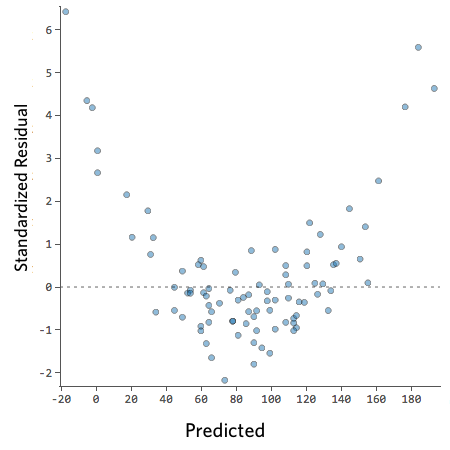
\includegraphics[width=6cm]{body/background/badresid.png}
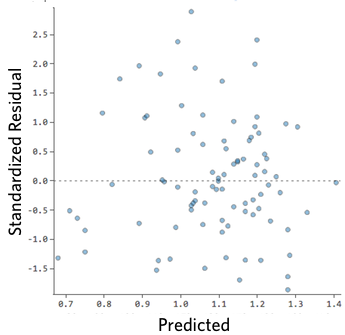
\includegraphics[width=6cm]{body/background/goodresid.png}
\caption[Plots of Residuals]{Two plots of residuals versus the explanatory variable, time. The figure on the left shows a residual plot that has a discernible quadratic pattern, suggesting a linear model is not a good fit. The figure on the right shows a residual plot that has no discernible pattern; that is it seems like random white noise that could have been sampled from a Gaussian distribution where the variance is independent from the prediction. This suggests a linear model is a good fit.}
\label{fig:resids}
\end{figure}

%http://docs.statwing.com/interpreting-residual-plots-to-improve-your-regression/

In some cases, a transformation from the original data to something more linear may be appropriate. For example, if the observed data is approximately exponential in nature, a log transformation would take the data from the log space to linear space, where a Least-Squares linear fit would be appropriate.

To generate the least squares line, we consider the following system of equations. In the following example, our explanatory variable is $t$, for time, and our response variable is $y$. We have $n$ discrete data points that are time/response pairs, and we are attempting to approximate $\alpha$ and $\beta$, the coefficients of the best fit line. 

The Mean Square Error, which is minimized in linear regression, is given by the following equation:

\begin{equation}
    \frac{1}{n}\sum_{i=1}^{n} (f(t_{i}) - y_{i})^2
\end{equation}

summed over all data points, where $y$ is the observation and $f(t)$ is the function of time evaluated at that point. From this equation, called the objective equation, we can find a solution that minimizes mean squared error. To find the coefficients of the least squares line, we use the following equations. 

\begin{equation}
H
=
\begin{bmatrix}
1 & t_{1} \\
1 & t_{2} \\
1 & t_{3} \\
\vdots & \vdots \\
1 & t_{n} 
\end{bmatrix}, \quad H\in\mathbb{R}^{n\times2}
\end{equation}

\begin{equation}
\bm{y}
=
H
\begin{bmatrix}
\alpha \\
\beta
\end{bmatrix}, \quad \bm{y}\in\mathbb{R}^n
\end{equation}

Here, $H$ is known as the design matrix. The first column vector is entirely 1's. The second column vector is all $n$ known time values ($x$). Setting up $H$ in this way makes it so Equation 2.8 is equivalent to 

\begin{equation}
    y_{i} = \alpha + \beta t_{i}
\end{equation}

which is the exact functional form we were looking for in Equation 2.5.

For each observation point, we have some relation between time and the response which we can estimate with these two equations. To estimate our final relationship, the coefficients $\hat{\alpha}$ and $\hat{\beta}$ are found with the following equation.

\begin{equation}
\begin{bmatrix}
\hat{\alpha} \\
\hat{\beta}
\end{bmatrix}
=
(H^{T}H)^{-1}H^{T}\bm{y}
\end{equation}

It should be noted that this example only involves prediction using a single input variable ($x$), however, the formulation is robust enough to be compatible with inputs of any dimension. Consider the case where the input is instead $X = (x_{1}, x_{2}, \hdots, x_{i})$, thus we now want to predict for the equation

\begin{equation}
    \bm{y} = \alpha + \beta X = \alpha + \beta_{1}\bm{x_{1}} + \beta_{2}\bm{x_{2}} + \hdots + \beta_{i}\bm{x_{i}}
\end{equation}

$H$ will then become 

\begin{equation}
H
=
\begin{bmatrix}
1 & x_{11} & x_{12} & \cdots & x_{1i} \\
1 & x_{21} & x_{22} & \cdots & x_{2i} \\
1 & x_{31} & x_{32} & \cdots & x_{3i} \\
\vdots & \vdots & \vdots & \ddots & \vdots \\
1 & x_{n1} & x_{n2} & \cdots & x_{in}
\end{bmatrix}
\end{equation}

and Equation 2.10 will become

\begin{equation}
\begin{bmatrix}
\hat{\alpha} \\
\hat{\beta_{1}} \\
\hat{\beta_{2}} \\
\vdots \\
\hat{\beta_{i}}
\end{bmatrix}
=
(H^{T}H)^{-1}H^{T}\bm{y}
\end{equation}

\subsection{Extensions of Linear Regression}

The variety of problems to which linear regression can be applied has created the need for various modifications to the technique. For example, there are some cases where certain points within a data set must be weighted more heavily than others. This cannot be done in a traditional least squares, but can be achieved through the introduction of an additional diagonal matrix $W$. For a matrix to be diagonal, it must only have entries along its main diagonal as seen in Equation 2.14. For this application, the time series data is always provided in chronological order with newer points coming last. For the purposes of prediction, we care more about the more recent data as initial behavior would be expected to be non-influential on end behavior. $W$ would then take the form

\begin{equation}
    W = diag(\lambda^{n}, \lambda^{n-1}, \cdots, \lambda^{1}) = 
    \begin{bmatrix}
    \lambda^{n} & 0 & 0 & \cdots & 0 \\
    0 & \lambda^{n-1} & 0 & \cdots & 0 \\
    0 & 0 & \ddots & \ddots & \vdots \\
    \vdots & \vdots & \ddots & \lambda^{1} & 0 \\
    0 & 0 & \cdots & 0 & \lambda^{0}
    \end{bmatrix}
\end{equation}

where $\lambda\in{[0,1]}$. $\lambda$ acts as a ``forgetting factor'', making the later occurring points exponentially more important in the parameter search. Effectively, this means the residual used in the MSE calculation from Equation 2.6 for each point is weighted by its associated power of $\lambda$ as in Equation 2.15. 

\begin{equation}
    \frac{1}{n}\sum_{i=1}^{n} (\lambda^{n-i}[f(t_{i}) - y_{i}])^2
\end{equation}

This allows for large residuals for the initial points while insisting on small residuals for the later points. The new equation to estimate the coefficients of our best fit line then becomes

\begin{equation}
\begin{bmatrix}
\hat{\alpha} \\
\hat{\beta}
\end{bmatrix}
=
(H^{T}WH)^{-1}H^{T}W\bm{y}
\end{equation}

As before, this function can also be used for a set of $i$ input variables reformatting the $H$ and coefficient matrices as in Equations 2.12 and 2.13.